\chapter{Geometric Classification}
\begin{commentbox}{IMPORTANT!}
    Before finidng support vectors, you must scale all attributes to have zero mean and unit variance, in order to match the canonical hyperplane. 
\end{commentbox}
\section{Support Vector Machines}
\begin{figure}[H]
    \centering
    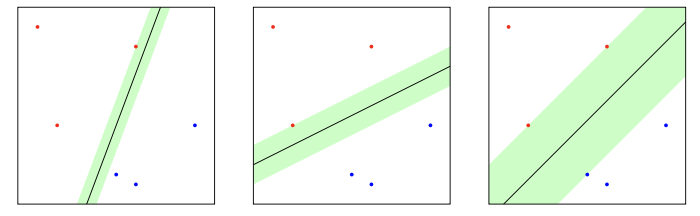
\includegraphics[width=0.75\linewidth]{img/svg_max_margin.png}
    \caption{Intuitively, in classification, a larger margin is better}
    \label{fig:svm_max_margin-label}
\end{figure}
\begin{figure}[H]
    \centering
    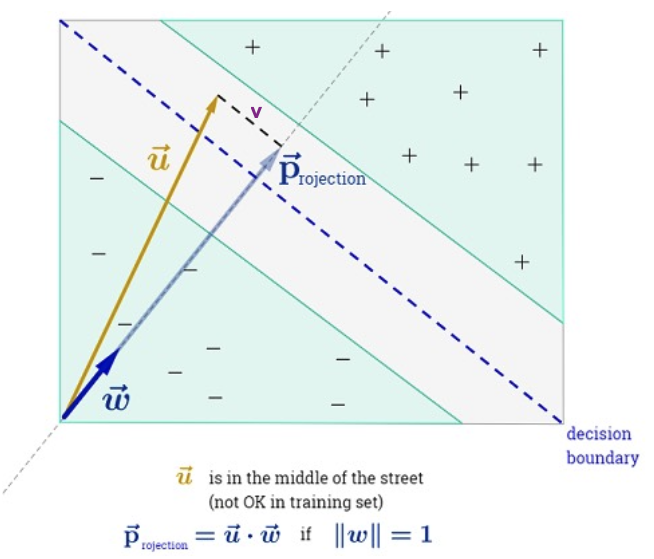
\includegraphics[width=0.5\linewidth]{img/middlestreet.png}
    \caption{For any $u$ during testing, our prediction is $sign(w\top u+ b)$}
    \label{fig:middlestreet-label}
\end{figure}

\subsection{Maximising the Margin}
\label{subsec:maximising_margin}

Intuitively, in classification tasks, a large margin between the classes is desirable as it may lead to better generalization from the training data to unseen data. This concept is often referred to as the ``widest street'' approach, where the margin is analogous to the width of the street. The goal of the SVM algorithm is to find the hyperplane that ``paves'' this widest street between the data points of different classes, hence maximising the margin.

\subsubsection*{Distance to a Hyperplane}
The distance from a point \( \mathbf{x} \) to a hyperplane defined by \( \mathbf{w}^T \mathbf{x} + b = 0 \) can be given by the formula:
\[
\text{Distance} = \frac{|\mathbf{w}^T \mathbf{x} + b|}{\|\mathbf{w}\|}.
\]
Here, the vector \( \mathbf{p}_{\mathbf{x}} \) represents the orthogonal projection of \( \mathbf{x} \) onto the hyperplane:
\[
\mathbf{p}_{\mathbf{x}} = \mathbf{x} - \frac{(\mathbf{w}^T \mathbf{x} + b)}{\|\mathbf{w}\|^2}\mathbf{w}.
\]
The vector \( \mathbf{x} - \mathbf{p}_{\mathbf{x}} \) is parallel to \( \mathbf{w} \) and thus orthogonal to the hyperplane, which confirms that \( \mathbf{p}_{\mathbf{x}} \) is indeed the orthogonal projection. Moreover, any vector \( \mathbf{u} \) in the hyperplane satisfies \( \mathbf{w}^T \mathbf{u} = 0 \) (orthogonal to \( \mathbf{w} \)), which underpins the definition of the orthogonal projection. The relationship between the norm of \( \mathbf{x} \) and its projection is:
\[
\|\mathbf{x}\|^2 = \|\mathbf{x} - \mathbf{p}_{\mathbf{x}} + \mathbf{p}_{\mathbf{x}}\|^2 = \|\mathbf{x} - \mathbf{p}_{\mathbf{x}}\|^2 + \|\mathbf{p}_{\mathbf{x}}\|^2,
\]
holding true by the Pythagorean theorem as \( \mathbf{x} - \mathbf{p}_{\mathbf{x}} \) and \( \mathbf{p}_{\mathbf{x}} \) are orthogonal.

\subsubsection*{Hard-Margin SVM}
In the context of SVMs, the points are separable if there exist weights \( \mathbf{w} \) and bias \( b \) such that \( y_i(\mathbf{w}^T \mathbf{x}_i + b) > 0 \) for each data point \( \mathbf{x}_i \) with label \( y_i \in \{-1, +1\} \). The margin of the SVM classifier is the minimum distance from any point to the hyperplane \( H(\mathbf{w}, b) \), defined as:
\[
\delta^* \equiv \min_i \frac{|\mathbf{w}^T \mathbf{x}_i + b|}{\|\mathbf{w}\|} = \min_i y_i\left(\frac{\mathbf{w}^T \mathbf{x}_i + b}{\|\mathbf{w}\|}\right).
\]
The points that lie exactly at distance \( \delta^* \) from the hyperplane are called support vectors. Therefore, a point \( \mathbf{x}^* \) is a support vector if and only if:
\[
\frac{|\mathbf{w}^T \mathbf{x}^* + b|}{\|\mathbf{w}\|} = \delta^*.
\]
The optimisation problem in SVMs is thus to maximise \( \delta^* \), the margin, by adjusting \( \mathbf{w} \) and \( b \), which geometrically corresponds to finding the widest possible street between the classes.

\begin{figure}[H]
    \centering
    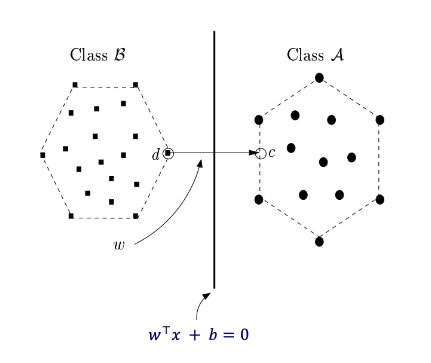
\includegraphics[width=0.5\linewidth]{img/convexhull.png}
    \caption{The two closest points of the convex hulls (the smallest convex set that contains all the points) determine the separating plane.}
    
\end{figure}
\subsection{Canonical Hyperplane}
There are many ways to describe a hyperplane, such that $H(w,b)$ and $H(\alpha w, \alpha b)$ will define the exact same set of points. 

To uniquely identify the separating hyperplane in SVM, we use the concept of a canonical hyperplane. A canonical hyperplane is defined such that for a given support vector \( \mathbf{x}^* \), the following condition holds:
\[
y^*(\mathbf{w}^T \mathbf{x}^* + b) = 1.
\]
This normalisation ensures that the distance from the support vector to the hyperplane is scaled such that it provides a consistent measure of confidence for predictions. The canonical form aids in the interpretation of SVM outputs, especially when comparing predictions for new data points.\\

Hence, for all support vectors, the above equation holds true, and for any other data point not on the margin boundary, the inequality \( y_i(\mathbf{w}^T \mathbf{x}_i + b) > 1 \) must be satisfied, as any point that is not the support vector must be farther away. This ensures that non-support vectors lie outside the margin defined by the support vectors. \\


For the remainder of the notes, it can be assumed that the margin for canonical hyperplanes is given by \( \delta^* = \frac{1}{\|\mathbf{w}\|} \), and it is this margin that we seek to maximise in SVM.\\

\subsubsection*{Maximum Margin Hyperplane}
The maximum margin hyperplane is the heart of the SVM classifier. The objective of SVM is to find the canonical hyperplane \( H(\mathbf{w}, b) \) which maximises the margin between the classes. The optimal hyperplane parameters \( (\mathbf{w}_*, b_*) \) are found by solving the following optimisation problem:
\[
(\mathbf{w}_*, b_*) = \arg\max_{\mathbf{w},b} \left\{ \frac{1}{\|\mathbf{w}\|} \right\} \text{ such that } y_i(\mathbf{w}^T \mathbf{x}_i + b) \geq 1, \forall i.
\]
This optimisation problem differs from the Perceptron algorithm, which continues to adjust its weights until all points are correctly classified, without necessarily maximizing the margin. The Perceptron stops as soon as it finds any solution that separates the data with zero error, without concern for the margin width or the generalisation of the classifier. In contrast, the SVM is designed to find the ``best'' solution by maximising the margin, leading to potentially better generalisation capabilities.

\subsection{Formulation of Hard-Margin SVM}
\label{subsec:formulation_hard_margin_svm}

The hard-margin SVM is formulated as an optimization problem where the goal is to minimize the norm of the weight vector \( \mathbf{w} \), which is directly related to maximizing the margin. The problem can be stated as:

\[
\text{minimize} \quad \frac{1}{2}\|\mathbf{w}\|^2
\]
\[
\text{subject to} \quad y_i(\mathbf{w}^T \mathbf{x}_i + b) \geq 1 \quad \text{for all} \quad i.
\]

The choice of \( \frac{1}{2} \) as a multiplier for the norm of \( \mathbf{w} \) is arbitrary and does not affect the solution; it is chosen for mathematical convenience as it simplifies the analysis, particularly when taking derivatives.\\

The choice of the squared Euclidean norm (Norm-2) over other norms (like the Manhattan norm, Norm-1) is not just for mathematical convenience.\\

Minimising the Euclidean Norm-2 tends to not penalise small values of \( \mathbf{w} \) as much, so they are not forced to approach zero, allowing all features to contribute.\\


Minimising the Manhattan Norm-1 treats all values equally, promoting sparsity in the solution, by penalising large and small values equally, akin to feature selection. \\

Usually in practice, minimising the squared Euclidean norm is less prone to overfitting compared to the Manhattan norm.

\subsubsection*{Lagrangian Formulation and the KKT Conditions}
The Lagrangian formulation introduces dual variables \( \alpha_i \) for each constraint in the optimisation problem, leading to the Lagrangian:
\[
L(\mathbf{w}, b, \boldsymbol{\alpha}) = \frac{1}{2}||\mathbf{w}||^2 + \sum_{i=1}^n \alpha_i[1 - y_i(\mathbf{w}^T \mathbf{x}_i + b)],
\]

where the goal is to minimise \( L \) with respect to \( \mathbf{w} \) and \( b \), and to maximise it with respect to the dual variables \( \alpha_i \geq 0 \).

The Karush-Kuhn-Tucker (KKT) conditions provide the necessary conditions for optimality in this context. They are given by:

\begin{align*}
\nabla_{\mathbf{w}}L &= \mathbf{w} - \sum_{i=1}^n \alpha_i y_i \mathbf{x}_i = 0  &\Rightarrow & \quad \mathbf{w} = \sum_{i=1}^n \alpha_i y_i \mathbf{x}_i, \\
\nabla_{b}L &= -\sum_{i=1}^n \alpha_i y_i = 0  &\Rightarrow & \quad \sum_{i=1}^n \alpha_i y_i = 0, \\
&\alpha_i[1 - y_i(\mathbf{w}^T \mathbf{x}_i + b)] = 0  &\Rightarrow & \quad \alpha_i = 0 \quad \text{or} \quad y_i(\mathbf{w}^T \mathbf{x}_i + b) = 1.
\end{align*}

Data points \( \mathbf{x}_i \) with corresponding \( \alpha_i \neq 0 \) are known as support vectors. These are the points that lie on the margin, and hence, \( y_i(\mathbf{w}^T \mathbf{x}_i + b) = 1 \) for support vectors. Importantly, the weight vector \( \mathbf{w} \) is expressed as a linear combination of the support vectors, showing the role they play in defining the decision boundary.

\begin{commentbox}{KKT Conditions}
The KKT conditions for optimality are a set of necessary conditions for a solution to be optimal in a mathematical optimisation problem. They are necessary and sufficient conditions for a local minimum in nonlinear programming problems.
\end{commentbox}

\begin{definitionbox}{Hard-SVM Dual Formulation}
    We can fine the dual-formulation for the Hard-SVM problem as follows:
    \[
    \max_\alpha\mathcal{L}(\alpha)\triangleq\sum_{i=1}^n\alpha_i-\frac12\sum_{i=1}^n\sum_{j=1}^ny_iy_j\alpha_i\alpha_jx_i^\top x_j
    \]

    subject to \[\alpha_{i}\geq0,\sum_{i=1}^{n}\alpha_{i}y_{i}=0.\]
    
\end{definitionbox}
In the context of SVMs, after solving for the Lagrange multipliers $\alpha_i^*$, the weight vector $\mathbf{w}^*$ and the bias term $b^*$ can be computed as follows:\\

The optimal weight vector is determined by the sum over all support vectors, denoted by non-zero $\alpha_i^*$, and is given by:
\[
\mathbf{w}^* = \sum_{i:\alpha_i^*>0} \alpha_i^* y_i \mathbf{x}_i
\]

The optimal bias term $b^*$ ensures that the decision boundary correctly classifies the support vectors. For any support vector $\mathbf{x}_i$, the following condition holds:
\[
y_i( (\mathbf{w}^*)^\top \mathbf{x}_i \rangle + b^*) = 1
\]
This can be rearranged to solve for $b^*$ using any support vector $\mathbf{x}_i$:
\[
b^* = \frac{1}{y_i} -  (\mathbf{w}^*)^\top\mathbf{x}_i = y_i - (\mathbf{w}^*)^\top\mathbf{x}_i
\]
Since all support vectors lie on the margin, and their $\alpha_i^*$ are non-zero, this formula will give the same result irrespective of the chosen support vector $\mathbf{x}_i$.\\

The above conditions provide a way to construct the separating hyperplane that maximises the margin between the two classes in the feature space, which is the essence of the hard-margin SVM.


\subsubsection*{Prediction with Hard-SVM}
Assume we fit our model to a training dataset, and want to make a new prediction for new data sample $x$. We predict $\hat{y} = 1$ if and only if $(w^*(^\top x + b^* >0$\\

We have
\begin{align*}
(w^{*})^{T}x+b^{*}& =\left(\sum_{i=1}\alpha_i^*y_ix_i\right)^{\prime}x+b^*  \\
&=\sum_{i=1:\alpha_i^*>0}^n\alpha_i^*y_i(x_i^Tx)+b^*
\end{align*}


\subsection{Soft-Margin SVM}

Sometimes, when data is non-linearly separable, we cannot guarantee points will be classified correctly such that $y_i(w^\top x_i+b)\geq1\text{ for all i}$. \\


In the soft-margin SVM, the introduction of slack variables \( \xi_i \) relaxes this condition, and allows some misclassifications. The optimisation problem can be written as:

\[
\min_{\mathbf{w},b,\boldsymbol{\xi}} \quad \frac{1}{2} \lVert \mathbf{w} \rVert^2 + C \sum_{i=1}^n \xi_i
\]

\[
\text{subject to} \quad y_i(\mathbf{w}^\top \mathbf{x}_i + b) \geq 1 - \xi_i \quad \text{and} \quad \xi_i \geq 0 \quad \forall i
\]

The parameter \( C \) in the soft-margin SVM controls the trade-off between maximising the margin and minimising the classification error. It enforces an upper bound on the norm of the weights.\\

A large C penalises even small margin violations, and a small C means we can freely violate the margin for some points as long as it helps make the margin wider. It provides a balance between minimising $||\textbf{w}||^2$\\ keeping a large margin, and minimising misclassified samples.\\

The Lagrangian of the soft-margin SVM is given by the hard-margin objective plus three additional terms incorporating the slack variables:

\[
\mathcal{L}(\mathbf{w}, b, \boldsymbol{\alpha}, \boldsymbol{\beta}) = \frac{1}{2} \lVert \mathbf{w} \rVert^2 +  \underbrace{C\sum_{i=1}^n \xi_i}_{\text{ soft margin }} - \sum_{i=1}^n \alpha_i [y_i(\mathbf{w}^\top \mathbf{x}_i + b) - 1 + \underbrace{\xi_i}_\text{ soft margin }] - \underbrace{\sum_{i=1}^n \beta_i \xi_i}_{\text{ soft margin }}
\]

To minimise in primal variables \( \mathbf{w}, b, \boldsymbol{\xi} \), and maximise in dual variables \( \boldsymbol{\alpha}, \boldsymbol{\beta} \geq 0 \), we apply the Karush-Kuhn-Tucker (KKT) conditions:

\begin{align*}
\nabla_{\mathbf{w}} \mathcal{L} &=  \mathbf{w} = \sum_{i=1}^n \alpha_i y_i \mathbf{x}_i = 0 \quad &\Rightarrow& \quad \mathbf{w} = \sum_{i=1}^n \alpha_i y_i \mathbf{x}_i\\
\nabla_b \mathcal{L} &= -\sum_{i=1}^n \alpha_i y_i = 0 \quad &\Rightarrow& \quad \sum_{i=1}^n \alpha_i y_i = 0\\
\nabla_{\xi_i} \mathcal{L} &= C - \alpha_i - \beta_i = 0 \quad &\Rightarrow& \quad C = \alpha_i + \beta_i\\
&\alpha_i (1 - \xi_i - y_i(\mathbf{w}^\top \mathbf{x}_i + b)) = 0 &\Rightarrow& \quad \alpha_i = 0\text{ or } y_i(\textbf{w}^\top x_i + b) = 1-\xi_i\\
&\beta_i \xi_i = 0 &\Rightarrow& \quad \beta_i = 0 \text{ or } \xi_i = 0
\end{align*}





The last two conditions above are known as the complementary slackness conditions. They imply that for any \( i \), either \( \alpha_i = 0 \) or \( y_i(\mathbf{w}^\top \mathbf{x}_i + b) = 1 - \xi_i \). Also, if \( \alpha_i = C \), then the corresponding point \( (\mathbf{x}_i, y_i) \) lies on or within the margin, or it is misclassified.\\

The introduction of the slack variable \( \xi_i \) in the soft-margin SVM leads to an additional constraint in the dual optimisation problem, which restricts the Lagrange multipliers for each data point:

\[
0 \leq \alpha_i \leq C
\]

This constraint ensures that the dual variables \( \alpha_i \) are bounded above by \( C \), reflecting the trade-off between margin width and classification error.

\begin{figure}[H]
    \centering
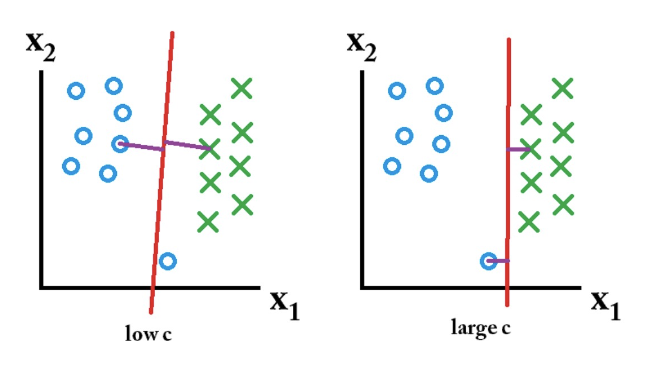
\includegraphics[width=0.5\linewidth]{img/large-small-margin.png}
    \caption{Comparing different effects of C sizes}
    
    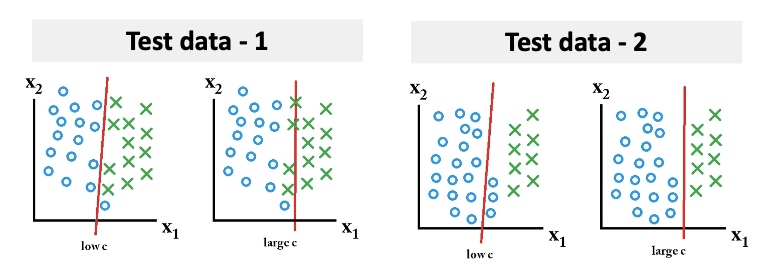
\includegraphics[width=0.8\linewidth]{img/svm_C.png}
    \caption{C is essentially a regularisation parameter, which controls the trade-off between: achieving a low error on the training data (larger C) and minimising the norm of the weights (smaller C). The most common method for finding appropriate C is cross validation.}
    
\end{figure}

Note that a soft-margin helps with in-training accuracy on data that can generally be linearly separable, but it alone cannot improve performance on data that that requires major feature space transformations.

\subsection{Soft-margin SVM Dual}

The dual formulation of the soft-margin SVM focuses on optimising the Lagrange multipliers \(\alpha_i\). The dual objective function to be minimised is:

\[
\mathcal{L}(\alpha) = \sum_{i=1}^{n} \alpha_i - \frac{1}{2} \sum_{i=1}^{n} \sum_{j=1}^{n} y_i y_j \alpha_i \alpha_j  \mathbf{x}_i^\top \mathbf{x}_j 
\]

This is subject to the constraints:

\[
0 \leq \alpha_i \leq C, \quad \text{and} \quad \sum_{i=1}^{n} \alpha_i y_i = 0
\]

From the dual variables, we can compute the weight vector \(\mathbf{w}^*\) as follows:

\[
\mathbf{w}^* = \sum_{i:\alpha_i^*>0} \alpha_i^* y_i \mathbf{x}_i
\]

The bias term \(b^*\) can be solved by using any support vector \(\mathbf{x}_i\) that lies on the margin, which is characterised by \(0 < \alpha_i < C\) and \(\xi_i = 0\). It is computed as:

\[
b^* = \frac{1}{y_i} - (\mathbf{w}^*)^\top \mathbf{x}_i = y_i - (\mathbf{w}^*)\top x_i
\]


Finally, classification of new samples can be performed using the sign of the decision function:

\[
\hat{y} = \text{sign}((\mathbf{w}^*)^\top \mathbf{x} + b^*)
\]

This formulation allows us to predict the class label of a new sample \(\mathbf{x}\) by considering the sign of the linear combination of the support vectors, weighted by the corresponding \(\alpha_i^*\), and adjusted by the bias term \(b^*\).


\subsection{Non-Linear Transformations and Kernels}

\subsubsection*{Intro to Kernels}
Kernel functions are a way of computing the dot product of two vectors $x$ and $y$ in some feature space, that could be possibly be very high dimensional. They are also called the `generalised dot product'. Intuitively, they are a similarity function that outputs a similarity score given two objects.

\begin{figure}[H]
    \centering
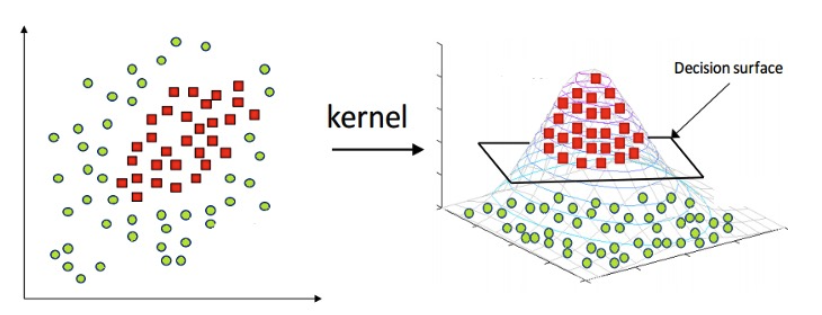
\includegraphics[width=0.5\linewidth]{img/kernel.png}
    
    
\end{figure}


In SVMs with non-linear transformations, the input data \( x \) is transformed into a higher dimensional space using a function \( \phi \). This enables the linear separation of data that is not linearly separable in the original input space. The transformed feature space is represented by \( z = \phi(x) \).\\

\subsubsection*{Lagrangian in Dual Form}

The dual formulation of the SVM with these transformations becomes (swapping $x_i$ with transformed $z_i$):

\[
\mathcal{L}(\alpha) = \sum_{i=1}^n \alpha_i - \frac{1}{2} \sum_{i=1}^n \sum_{j=1}^n y_i y_j \alpha_i \alpha_j z_i^\top z_j
\]

subject to:

\[
0 \leq \alpha_i \leq C, \quad \sum_{i=1}^n \alpha_i y_i = 0.
\]

\subsubsection*{Classification in SVM}

To classify new samples, we use the decision function:

\[
g(x) = \text{sign}(w^\top z + b)  = \text{sign} \left( \sum_{i:\alpha_i>0, z_i \text{is support vector}} \alpha_i y_i z_i^\top z + b \right),
\]

where \( b \) is calculated from any support vector \( z_i \):

\[
b = 1 - y_i w^\top z_i.
\]


So to solve this problem all we need is the transformed data in the form $z_i^\top z_j$.\\

\subsubsection*{The Kernel Function}

The kernel function is defined as the dot product of two distinct transformed vectors of $\textbf{x}$:
\begin{equation*}
    K(\mathbf{x}, \mathbf{x'}) = \langle \phi(\mathbf{x}), \phi(\mathbf{x'}) \rangle = \mathbf{z}^\top \mathbf{z}'
\end{equation*}
where $\phi$ is a transformation that maps the input data to a higher-dimensional space, and $\langle \cdot, \cdot \rangle$ denotes the inner product.

\subsubsection*{Polynomial Kernel Function Example}
Consider a two-dimensional input vector $\mathbf{x} = (x_1, x_2)$. We also have a polynomial transform of degree 2:
\begin{align*}
    \mathbf{z} &= \phi(\mathbf{x}) = (1, x_1, x_2, x_1^2, x_2^2) \\
\end{align*}
The polynomial kernel of degree 2 is given by:
\begin{align*}
    K(\mathbf{x}, \mathbf{x'}) = \mathbf{z}^\top \mathbf{z} &= 1 + x_1x_1' + x_2x_2' + x_1^2{x_1'}^2 + x_2^2{x_2'}^2
\end{align*}


We can also derive kernels straightaway and work out $\textbf{z}$ later:
\begin{align*}  K(\mathbf{x},\mathbf{x}^{\prime})& =(1+\mathbf{x}^\top\mathbf{x}^\prime)^2=(1+x_1x_1^\prime+x_2x_2^\prime)^2  \\
&=1+x_1^2{x_1^{\prime}}^2+x_2^2{x_2^{\prime}}^2+2x_1x_1^{\prime}+2x_2x_2^{\prime}+2x_1x_2x_1^{\prime}x_2^{\prime}
\end{align*}

The inner product for $\textbf{z}$ is:
\begin{equation*}
    \mathbf{z} = (1, x_1^2, x_2^2, \sqrt{2}x_1, \sqrt{2}x_2, \sqrt{2}x_1x_2)
\end{equation*}




\subsubsection*{Linear Kernel Example}
The linear kernel is simply the dot product in the input space, representing the similarity of $\mathbf{x}$ and $\mathbf{x'}$:
\begin{equation*}
    K(\mathbf{x}, \mathbf{x'}) = \mathbf{x}^\top \mathbf{x'}
\end{equation*}


\subsubsection*{Properties of Kernel Functions}

\begin{itemize}
    \item Kernels provide a compact representation of the data in the transformed feature space.
    \item The choice of kernel is task-specific and greatly influences the performance of the SVM.
    \item The best way to determine the appropriate kernel and its parameters is through cross-validation.
\end{itemize}

The kernel function \( K(x, x') \) replaces the dot product in the feature space, allowing us to compute the similarity between two points in the original input space without explicitly computing their coordinates in the feature space. \\


Kernels can be understood as a compact representation of the classification task's knowledge, encapsulating the structure of the data in the transformation \( \phi \) that they implicitly apply. The choice of kernel is task-specific and often determined through cross-validation to achieve the best classification performance.\\

Non-linear kernels like the polynomial kernel allow more complex relationships by considering not just the direct similarity but also the interactions between the features of \( \textbf{x} \) and \( \textbf{x'} \).

\subsubsection*{Gaussian (Radial Basis Function -  RBF) Kernel}

Consider this feature map in $\mathbb{R}$:

\[
\phi(x)_n=\frac1{\sqrt{n!}}\exp-x^2/2x^n
\]

\[
\begin{aligned}
\phi(x)^T\phi(x^{\prime})& =\sum_{n=0}^\infty\left(\frac1{\sqrt{n!}}e^{-x^2/2}x^n\right)\left(\frac1{\sqrt{n!}}\mathrm{e}^{-(x^{\prime})^2/2}(x^{\prime})^n\right)  \\
&=e^{-\frac{x^2+(x^{\prime})^2}2}\sum_{n=0}^\infty\frac{(x\cdot x^{\prime})^n}{n!} \\
&=e^{-\frac{\|x-x^{\prime}\|^2}2}
\end{aligned}
\]

In this kernel, we take the squared distance between two datapoints instead of their dot product(s) as seen in the polynomial kernel. So the amount of influence one observation has on another is a function of the squared distance. \\

Intuitively we can see if the distance between them two datapoints are greater, the less influence they have on each other, because the kernel function evaluates to a smaller value (due to a negative sign in the power). This makes Gaussian RBF act a bit like a Nearest Neighbour classification.

We can further scale this influence by a factor $\gamma$ from cross validation:
\[K(x,x')=\exp\left(-\gamma\underbrace{\|x-x'\|^2}_{radial}\right)\]\\

\subsubsection*{SVM Predictor for Gaussian RBF}

THe SVM predictor for the Gaussian RBF can be written as:

\[g(x)=\text{sign}\left(\sum_{x_i\text{is SV}}\alpha_iy_iK(x_i,x)+b\right)=\text{sign}\left(\sum_{x_i\text{is SV}}\alpha_iy_ie^{-\gamma\|x-x_i\|^2}+b\right)\]

\begin{sidenotebox}{RBF as an Infinite Sum}
    It is also interesting to note that the Radial Basis Function is setting the polynomial kernel to infinite dimensions without a constant:\\

To express the Gaussian RBF as an infinite sum of polynomial kernels, we can use the Taylor series expansion of the exponential function. The exponential function can be expanded as:
\begin{equation*}
e^z = \sum_{n=0}^{\infty} \frac{z^n}{n!}
\end{equation*}

Applying this to the Gaussian RBF kernel, we substitute \( z \) with \( -\gamma \|\mathbf{x} - \mathbf{x}'\|^2 \), yielding:
\begin{equation*}
e^{-\gamma \|\mathbf{x} - \mathbf{x}'\|^2} = \sum_{n=0}^{\infty} \frac{(-\gamma \|\mathbf{x} - \mathbf{x}'\|^2)^n}{n!}
\end{equation*}

This infinite series is a sum of polynomial terms of increasing degree, weighted by the factor \( \frac{(-\gamma)^n}{n!} \), and constitutes the Gaussian RBF kernel as an infinite sum of polynomial kernels.

\end{sidenotebox}

\subsection{The Kernel Trick in Support Vector Machines}

The kernel trick is a method used in SVMs to solve non-linear classification problems. It allows us to operate in the original input space without explicitly computing the coordinates in a higher-dimensional space.


\subsubsection*{Computational Benefits of the Kernel Function}
A kernel function like:
\begin{equation*}
K(\mathbf{x}, \mathbf{x}') = (c + \mathbf{x}^\top \mathbf{x}')^q = \left( c + \sum_{j=1}^{d} x_j x_j' \right)^q
\end{equation*}
will have \( d^q \) terms if expanded. The kernel trick avoids this explicit expansion, thus offering computational benefits.

\subsection{Choosing Kernels}
In kernel learning, we have:
\begin{itemize}
    \item A kernel function \( K_j(\mathbf{x}, \mathbf{x}') = \phi_j(\mathbf{x})^\top \phi_j(\mathbf{x}') \) and a combined kernel \( K(\mathbf{x}, \mathbf{x}') = \sum_{j=1}^{J} \gamma_j K_j(\mathbf{x}, \mathbf{x}') \) where \( \gamma_j \) are the coefficients for each kernel \( K_j \).
    \item This is equivalent to having a feature vector \( \mathbf{z} = (\phi_1, \ldots, \phi_J) \) and a weight vector \( \mathbf{w} = (w_1, \ldots, w_J) \).
    \item To limit the number of kernels used, a penalty is imposed by minimizing \(\left( \sum_{j=1}^{J} \|\mathbf{w}_j\|^p \right)^{2/p}\) for \( p \leq 2 \), which is a mixed \( L_1-L_2 \) penalty for \( p = 1 \).
\end{itemize}

\subsubsection*{Training Time and Optimisation}
\begin{itemize}
    \item Training time with Quadratic Programming (QP) is typically \( O(n^3) \), but can be much faster with Gradient Descent (GD) or Stochastic Gradient Descent (SGD) when seeking an approximate solution.
\end{itemize}

The kernel \( K \) must compute inner products in the feature space \( \mathcal{Z} \), such that \( K(\mathbf{x}, \mathbf{x}') = \mathbf{z}^\top \mathbf{z}' \).

\subsubsection*{Consequences}
\begin{itemize}
    \item The kernel matrix \( K_{x_1,\ldots,x_n} \) is symmetric and positive semidefinite, satisfying Mercer's condition.
    \item For any \( \mathbf{x}_1, \ldots, \mathbf{x}_n \), the kernel matrix is given by:
\end{itemize}
\begin{equation}
K_{x_1,\ldots,x_n} = 
\begin{bmatrix}
K(\mathbf{x}_1, \mathbf{x}_1) & \cdots & K(\mathbf{x}_1, \mathbf{x}_n) \\
\vdots & \ddots & \vdots \\
K(\mathbf{x}_n, \mathbf{x}_1) & \cdots & K(\mathbf{x}_n, \mathbf{x}_n)
\end{bmatrix}
\end{equation}

\subsubsection*{Mercer's Condition}
If \( \mathbf{z}^T = (z_1, \ldots, z_n) \), then \( K_{x_1,\ldots,x_n} = \mathbf{ZZ}^\top \) and for any vector \( \mathbf{u} \), we have:
\begin{equation}
\mathbf{u}^\top K_{x_1,\ldots,x_n} \mathbf{u} = \mathbf{u}^\top \mathbf{ZZ}^\top \mathbf{u} = (\mathbf{Z}^\top \mathbf{u})^\top (\mathbf{Z}^\top \mathbf{u}) = \|\mathbf{Z}^\top \mathbf{u}\|^2 \geq 0
\end{equation}

\subsubsection*{Sufficiency of Mercer's Condition}
The existence of \( \mathcal{Z} \) is guaranteed as long as Mercer's conditions are satisfied. This allows us to work with kernel functions without explicitly computing the feature mappings.

\subsubsection{Overfitting in Gaussian RBF}
Below is an example of how increasing the Gaussian RBF's $\gamma$ parameter leads to overfitting, cross-validation is vital to prevent such occurrences.
\begin{figure}[H]
\centering
\begin{subfigure}{.5\textwidth}
  \centering
  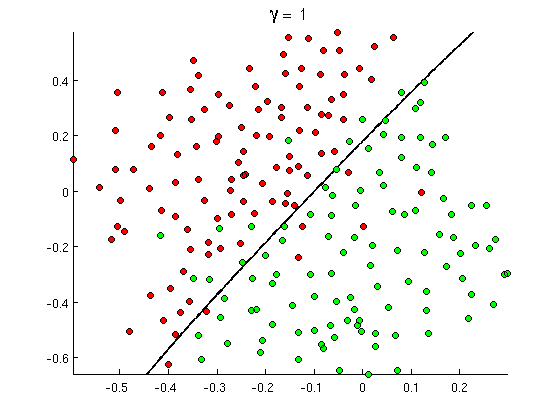
\includegraphics[width=.95\linewidth]{img/rbf1.png}
  \caption{Gaussian RBF with $\gamma = 1$, accuracy 91.9\%}
  \label{fig:rbf1}
\end{subfigure}%
\begin{subfigure}{.5\textwidth}
  \centering
  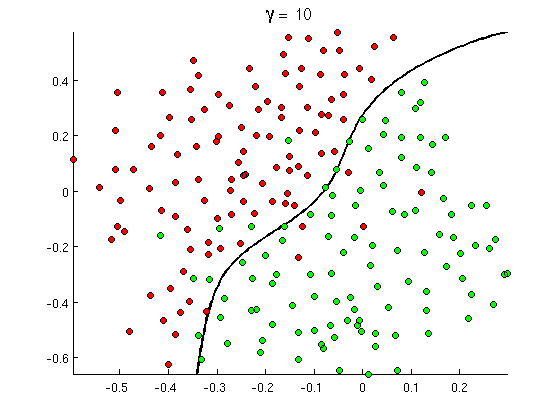
\includegraphics[width=.95\linewidth]{img/rbf2.png}
  \caption{Gaussian RBF with $\gamma = 10$, accuracy 93.3\%}
  \label{fig:rbf2}
\end{subfigure}
\newline
\begin{subfigure}{.5\textwidth}
  \centering
  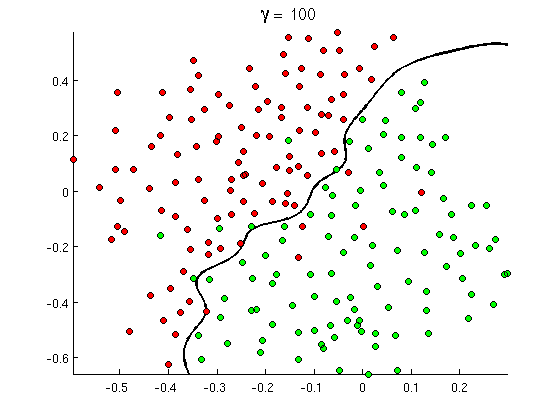
\includegraphics[width=.95\linewidth]{img/rbf3.png}
  \caption{Gaussian RBF with $\gamma = 100$, accuracy 93.4\%}
  \label{fig:rbf3}
\end{subfigure}%
\begin{subfigure}{.5\textwidth}
  \centering
  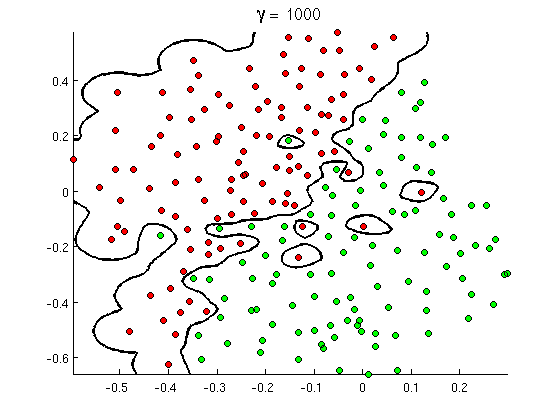
\includegraphics[width=.95\linewidth]{img/rbf4.png}
  \caption{Gaussian RBF with $\gamma = 1000$, accuracy 100\% (overfit!)}
  \label{fig:rbf4}
\end{subfigure}
\caption{Visualisation of the Gaussian RBF kernel with various $\gamma$ parameters}
\label{fig:rbf}
\end{figure}

\subsection{VC-Dimension for SVM}
\begin{enumerate}
    \item The SVM model is inherently linear:
    \begin{itemize}
        \item The number of parameters in the model is equal to the dimension of the data plus one (for the bias term), i.e., \( d+1 \).
    \end{itemize}
    \item The objective of the SVM is to maximise the margin:
    \begin{itemize}
        \item This is the distance between the separating hyperplane and the nearest data points from each class, which are known as support vectors.
        \item Among all possible lines/hyperplanes that perfectly separate the data, the SVM selects the one with the maximum margin.
    \end{itemize}
\end{enumerate}

These properties significantly reduce the hypothesis space by eliminating a vast number of potential candidates which do not meet the margin criterion. Consequently:

\begin{itemize}
    \item The hypothesis space of SVMs has a very small Vapnik-Chervonenkis (VC) dimension, which is indicative of the model's capacity to learn a variety of functions.
    \item A smaller VC dimension and growth function imply that SVMs can achieve better generalisation on unseen data, which is the ability to perform well on new inputs not present in the training data.
\end{itemize}



\begin{figure}[H]
    \centering
    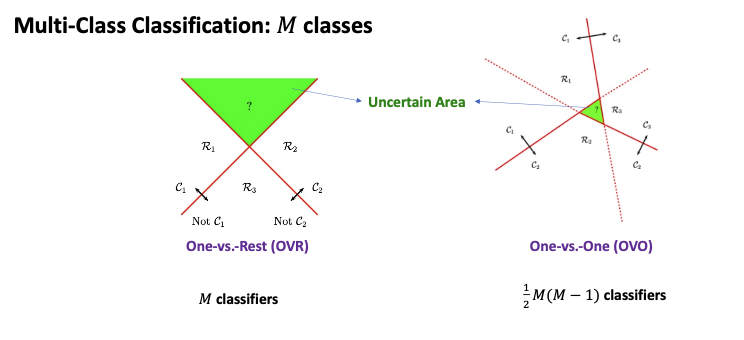
\includegraphics[width=0.75\linewidth]{img/multiclass.png}
\end{figure}


\section{K-Nearest-Neighbours}